\documentclass{ltjsarticle}

\usepackage{amsmath}
\usepackage{amssymb}
\usepackage{amsthm}
\usepackage{ mathrsfs }
\usepackage{enumerate}
\usepackage{bbm}
\usepackage{lipsum}
\usepackage{fancyhdr}
\usepackage{tikz-cd} 
\usetikzlibrary{graphs}
\usepackage{luatexja-ruby} 
\usepackage{graphicx} 
\graphicspath{ {./images/} }

\newtheorem{theorem}{定理}[section] 
\newtheorem{proposition}{命題}[section] 
\newtheorem{definition}{定義}[section] 
\newtheorem{problem}{例題}
\newtheorem{exercise}{問題}
\newtheorem{postulate}{公準}[section] 
\newtheorem{lemma}{補題}[section] 
\newtheorem{notation}{記法}[section] 
\newtheorem{remark}{注釈}[section] 
\newtheorem{corollary}{系}[section] 
\newtheorem{terminology}{Terminology}[section] 
\newtheorem{example}{例}[section] 
\newtheorem{step}{手順} 
\newtheorem{solution}{解答}[section] 
\newtheorem{fact}{事実}[section] 


\DeclareMathOperator{\diam}{diam}
\DeclareMathOperator{\Gal}{Gal}
\DeclareMathOperator{\rank}{rank}
\DeclareMathOperator{\Hom}{Hom}
\DeclareMathOperator{\Dom}{Dom}
\DeclareMathOperator{\Ann}{Ann}
\DeclareMathOperator{\grad}{grad}
\DeclareMathOperator{\Span}{Span}
\DeclareMathOperator{\interior}{int}
\DeclareMathOperator{\ind}{ind}
\DeclareMathOperator{\supp}{supp}
\DeclareMathOperator{\ob}{ob}
\DeclareMathOperator{\Spec}{Spec}
\DeclareMathOperator{\MaxSpec}{MaxSpec}
\DeclareMathOperator{\PreSh}{PreSh}
\DeclareMathOperator{\Sh}{Sh}
\DeclareMathOperator{\Fun}{Fun}
\DeclareMathOperator{\Ext}{Ext}
\DeclareMathOperator{\Aut}{Aut}
\DeclareMathOperator{\Ker}{Ker}
\DeclareMathOperator{\Image}{Im}
\DeclareMathOperator{\Coker}{Coker}
\DeclareMathOperator{\id}{id}
\DeclareMathOperator{\Mod}{Mod}
\DeclareMathOperator{\QCoh}{QCoh}
\DeclareMathOperator{\Coh}{Coh}
%\newcommand*{\name}[\num_arguments][default values]{{\color{#1}\Large #2}}
\newcommand*{\Z}{\mathbb{Z}}
\newcommand*{\Q}{\mathbb{Q}}
\newcommand*{\R}{\mathbb{R}}
\newcommand*{\multivar}[2]{{#1_1,\cdots,#1_{#2}}}
\newcommand*{\localization}[2]{#1_{\mathfrak{#2}}}
\newcommand*{\ringedspacemorph}[1]{(#1,#1^{\#})}
\newcommand*{\sheaf}[2]{(#1,{\mathcal{#2}}_{#1})}
\newcommand{\fib}[1]{%
  \mathbin{\mathop{\times}\limits_{#1}}%
}
\newcommand{\tens}[1]{%
  \mathbin{\mathop{\otimes}\displaylimits_{#1}}%
}
\title{常微分方程式と物理学}
\author{ボン補習校高校数学}
\date{}

% Taylor expansion and Euler's identity
% 
% Schrodinger's equation
% Gaussian integration and probability theory introduction with some example random variable

\begin{document}

\maketitle


このコースのゴールはシュレディンガー方程式の導出とマクスウェル方程式を用いた特殊相対性理論の光速度不変の原理の証明です。

\section{極限の定義と微分}
人間の体はこの世界のことを知るには全く性能が足りません。この世界を作り出した知性がいるとするならば、人間の能力は憶えられる量も目で終える物体のスピードも、理解できる物事の種類も創造主に遠く及ばないでしょう。しかし、科学者たちは知恵を絞って我々が知れる、理解できる物事の数をどうやって増やせるのかを考えてきました。
\par 微分とは自然科学における顕微鏡です。生物の体は複雑ですが、顕微鏡で見ると小さなより単純な細胞の集まりだということがわかります。微分は数学における小さな細胞を調べるための道具を与えてくれます。数学における細胞とはズバリまっすぐな線です。人間の知能ではまっすぐなもの以外理解することが難しいですが、まっすぐな世界の知識を使ってどうやって曲がった世界のことを知れるのかを学んでいきます。
\subsection{集合}

\begin{definition}
集合とは数や図形、文字などをまとめて集りのことである。
\end{definition}

\begin{example}
整数全ての集合を$\Z$、有理数全ての集合を$\Q$、実数すべての集合を$\R$と書きます。
\end{example}

上の集合は全て無限の数の集まりですが、有限の数の集まりを考えることもあります。例えば$1$から$10$の数の集まりを
\begin{equation*}
\{1,2,3,4,5,6,7,8,9,10\}
\end{equation*}
というように書いたりします。またいくつかの数字を消したいとき。例えば$10$を消して$1$から$9$までの数の集まりを書くときは
\begin{equation*}
\{1,2,3,4,5,6,7,8,9\}=\{1,2,3,4,5,6,7,8,9,10\}\backslash\{10\}
\end{equation*}
というように書いたりします。
\begin{example}
$0$以外の整数全体の集合を$\Z\backslash\{0\}$と書いたりします。
\end{example}
\subsection{極限}
\begin{definition}
関数$f(x)$において、定義域とは$x$に代入できる全ての数の集合である。
\end{definition}

\begin{example}
次のような関数を考える。
\begin{equation*}
f(x) = {\frac {(x-1)(x+1)} {(x+1)}}
\end{equation*}
$x$に$-1$を代入すると。
\begin{equation*}
f(x) = {\frac {-2\times 0} {0}}
\end{equation*}
となり、$0$で割り算をしなくてはいけなくなります。よってこの関数の定義域は$-1$以外の全ての実数。よって
\begin{equation*}
\R\backslash\{-1\}
\end{equation*}
のようにかけます。
\end{example}

上の例では式を約分することにより関数を次のように表すことができます。
\begin{equation*}
f(x) = {\frac {(x-1)(x+1)} {(x+1)}}=(x-1)
\end{equation*}
数学では指定された書き方が重要なのでこの関数の定義域は$\R\backslash\{0\}$ですが、この形に注目すると$x=-1$の時の計算ができるようになります。このように最初の形では計算できないけれども、少し形を変えてあげることで計算できるようになる時、「本当はやってはいけないかもしれない」ということを強調するために
\begin{equation*}
\lim_{x\to-1}f(x) = \lim_{x\to-1}{\frac {(x-1)(x+1)} {(x+1)}} =\lim_{x\to-1}(x-1)= -2
\end{equation*}
というふうに書きます。

\begin{problem}
次の極限を計算せよ。
\begin{equation*}
\lim_{x\to 0} x, \quad\lim_{x\to 0} {\frac {x^2} x}, \quad\lim_{x\to 2} {\frac {(x-2)(x+2)}{x-2}}
\end{equation*}
\end{problem}

\subsection{$x^n$の微分}

最初に紹介した通り、まっすぐな世界を使って曲がった世界のことを調べることが微分のゴールです。二次関数を考えてみましょう。
\begin{center}
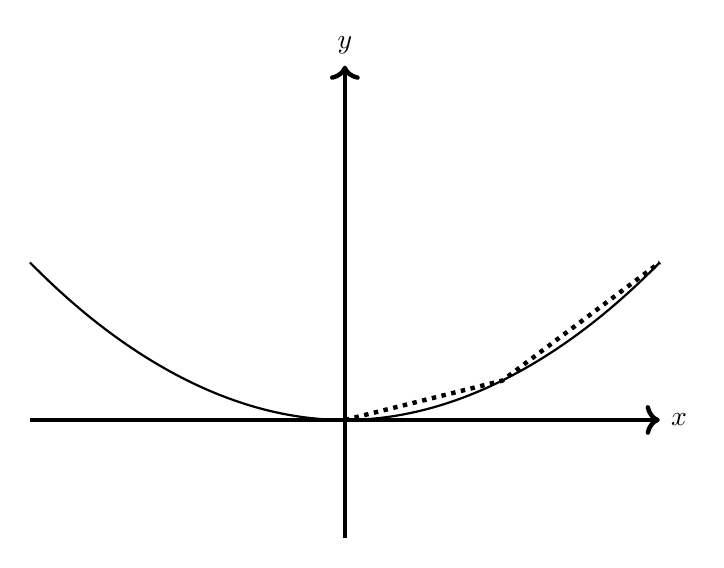
\begin{tikzpicture}
\draw[->,ultra thick] (-4,-1.5)--(4,-1.5) node[right]{$x$};
\draw[->,ultra thick] (0,-3)--(0,3) node[above]{$y$};
\draw[thick]  (0,-1.5) parabola (4,0.5);
\draw[thick] (0,-1.5) parabola (-4,0.5);
\draw[ultra thick, dotted] (0,-1.5) -- (2,-1)--(4,0.5);
\end{tikzpicture}
\end{center}

昔の人は曲がった図形は扱いにくいので、このように直線で形を似せることで計算を楽にしていました。しかし、正確にしようとすればするほど、線が折れている場所を増やす必要があり、どんどん難しくなっていきます。ここで発想を逆転させます。「調べたい部分が小さければ小さいほど、必要な折れた線の数は少なくなるのではないか。」ここで調べたい部分を限りなく小さくすることで、たった一つの直線で正確な計算をできるようにする。これが微分のアイデアです。
\par このアイデアは何も特別なものではなく、私たちは同じような現象を毎日見ています。地球は本当は丸いボールのような形ですが、私たちの見える世界はとても狭いので、小さな範囲では平らな世界に見えます。
\par 実際に計算してみましょう。下の図で$h$を限りなく小さくすると、

\begin{center}
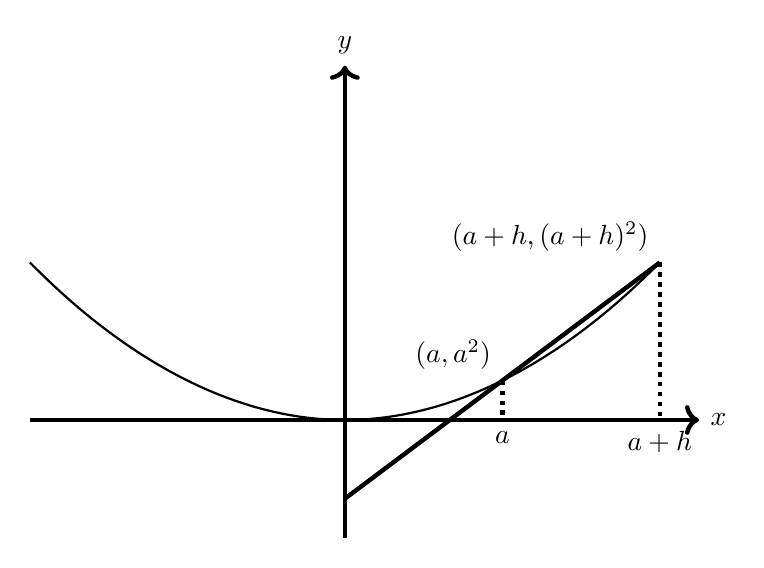
\begin{tikzpicture}
\draw[->,ultra thick] (-4,-1.5)--(4.5,-1.5) node[right]{$x$};
\draw[->,ultra thick] (0,-3)--(0,3) node[above]{$y$};
\draw[thick]  (0,-1.5) parabola (4,0.5);
\draw[thick] (0,-1.5) parabola (-4,0.5);
\draw[ultra thick] (0,-2.5) -- (4,0.5);
\draw[ultra thick, dotted] (2,-1)node[above left]{$(a,a^2)$}--(2,-1.5)[below]node{$a$};
\draw[ultra thick, dotted] (4,0.5)node[above left]{$(a+h,(a+h)^2)$}--(4,-1.5)[below]node{$a+h$};
\end{tikzpicture}
\end{center}
から
\begin{center}
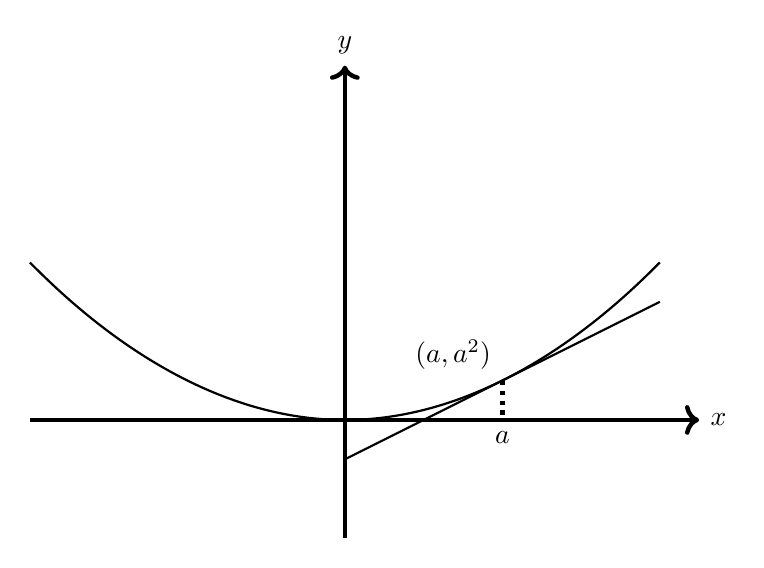
\begin{tikzpicture}
\draw[->,ultra thick] (-4,-1.5)--(4.5,-1.5) node[right]{$x$};
\draw[->,ultra thick] (0,-3)--(0,3) node[above]{$y$};
\draw[thick]  (0,-1.5) parabola (4,0.5);
\draw[thick] (0,-1.5) parabola (-4,0.5);
\draw[thick] (0,-2)--(2,-1) -- (4,0);
\draw[ultra thick, dotted] (2,-1)node[above left]{$(a,a^2)$}--(2,-1.5)[below]node{$a$};
\end{tikzpicture}
\end{center}
のように二次関数にピッタリとくっつく線が描けます。この直線は$(a,a^2)$を通ります。必要なのは傾きだけです。これを計算してみましょう。つぎの公式を使います。
\begin{equation*}
(a+b)^2 = a^2+2ab+b^2
\end{equation*}

これを使うと

\begin{align*}
(a+h)^2 = a^2+2ah+h^2
\end{align*}
よって最初の図において傾きは
\begin{equation*}
{\frac {(a+h)^2-a^2} {h}} 
\end{equation*}
$h$が限りなく小さくなると、
\begin{equation*}
\lim_{h\to0} {\frac {(a+h)^2-a^2} {h}} = \lim_{h\to0}{\frac {2ha+h^2} h} = \lim_{h\to0}2a+h = 2a
\end{equation*}
よってこの線は
\begin{equation*}
y - a^2 = 2a(x-a)
\end{equation*}
というように計算できます。このことをまとめましょう。
\begin{definition}
$f(x)$の$a$における微分とは
\begin{equation*}
{\frac {df} {dx}}(a) = \lim_{h\to0}{\frac {f(a+h)-f(a)} h}
\end{equation*}
である。
\end{definition}

\par\textbf{問題2積の微分}
\par 二つの関数$f,g$を考える。${\frac {df} {dx}}(a),{\frac {dg} {dx}}(a)$が計算できるとして。つぎの微分をこの二つで表す方法を考える。
\par\textbf{ステップ１}
\begin{equation*}
{\frac {d(fg)} {dx}}(a) 
\end{equation*}
の定義を書け。
\par\textbf{ステップ２}
\begin{equation*}
f(a+h)g(a+h) -f(a)g(a) = f(a+h)g(a+h)-f(a)g(a+h)+f(a)g(a+h)-f(a)g(a)
\end{equation*}
と$f(a),g(a)$が定数であることに注意し、また$\lim_{h\to 0}$と足し算掛け算が交換できることにより、
\begin{equation*}
{\frac {d(fg)} {dx}}(a)  = {\frac {df} {dx}}(a)g(a)+f(a){\frac {dg} {dx}}(a)
\end{equation*}
を証明せよ。（ヒント：$f,g$の微分の定義を書いてみよう。）

\section{極限と連続関数}

\begin{definition}
数列とは$\{a_1,a_2,\cdots,a_n,\cdots\}$のように自然数$1,2,3,\cdots$で番号がつけられた数の集まりのことである。
\end{definition}

\begin{example}数列には次のようなものがある。
\begin{enumerate}[1).]
\item $1,5,9,13,\cdots$前の数に$4$を足してできる数列。（公差が$4$の等差数列）
\item $1,2,4,8,16,\cdots$前の数に$2$をかけてできる数列。（公比が$4$の等比数列）
\item $1,{\frac 1 2},{\frac 1 4},{\frac 1 8},{\frac 1 16},\cdots$前の数に${\frac 1 2}$をかけてできる数列。（公比が${\frac 1 2}$の等比数列）
\item $1,1,2,3,5,8,\cdots$一つ前と二つ前の数を足してできる数列。（フィボナッチ数列）
\end{enumerate}
\label{example_sequences}
\end{example}

数列とは、特定の数$n$を別の数$a_n$に対応させること、つまり$n$についての関数として考えることができます。
\begin{example}それぞれ例\ref{example_sequences}の四つの数列は次の関数で表されます。
\begin{enumerate}[1).]
\item 公差が$4$の等差数列 $a_n = 4n-3$
\item 公比が$4$の等比数列 $a_n = 4^{n-1}$
\item 公比が${\frac 1 2}$の等比数列 $a_n = \left({\frac 1 2}\right)^{n-1}$
\item フィボナッチ数列 $a_n = {\frac 1 {\sqrt{5}}}\left(\left({\frac {1+\sqrt{5}} 2}\right)^n-\left({\frac {1-\sqrt{5}} 2}\right)^n\right)$
\end{enumerate}
\end{example}

例えば最初の例のように$1001$番目はと聞かれたら$1$に$4$を$1000$回足して、$4001$になります。三番目の場合は$11$番目は${\frac 1 {1024}}$そして$18$番目は${\frac 1 {131072}}$となります。これを少数にして書くと、
\begin{equation*}
{\frac 1 {1024}}\approx0.0009765625,\quad{\frac 1{131072}} \approx 0.00000762939,
\end{equation*}
のようにどんどん小さくなるのがわかると思います。これを続けていくと最終的に$0$になることが予想されます。

\begin{definition}
$(a_n)_{n=1,2,\cdots}$を数列とする。
\begin{equation*}
\lim_{n\to\infty} a_n = \alpha
\end{equation*}
とは$n$を大きくするとどんどん$\alpha$に近づいていくことである。
\end{definition}

\begin{remark}
二つの数字の距離は絶対値$\vert\quad\vert$で計算することができます。$\alpha$に近づくというのは数列の数$a_n$と$\alpha$の距離
\begin{equation*}
\vert a_n-\alpha\vert
\end{equation*}
が小さくなることだと言えます。つまり$\alpha$と$(a_n)_{n=1,2,\cdots}$の隙間を好きなだけ小さくできる。よって
\begin{equation*}
\text{どんなに小さな$\alpha$の周りの隙間にも無限の数列の数$a_n$が存在する}
\end{equation*}
というような言い換えを定義として数学では使います。
\end{remark}

\begin{exercise}
次の数列を$1$から$5$番目の数字を書きましょう。また例\ref{example_sequences}三番と同じ考え方で数列の極限を求めましょう。
\begin{equation*}
a_n={\frac 1 n}
\end{equation*}
\end{exercise}

\begin{proposition}
$a,b,c$を実数とすると次のことが成り立つ。
\begin{equation*}
\vert a+b\vert < c\text{　が正しいならば　}a+b<c\text{　も正しい。}
\end{equation*}
また
\begin{equation*}
\vert ab+ac\vert =\vert a\vert\times\vert b+c\vert
\end{equation*}
も成り立つ。
\label{proposition_absolute_value_properties}
\end{proposition}

\begin{proposition}
$a,b$を実数とすると次のことが成り立つ。
\begin{equation*}
\vert a+b\vert \leq \vert a\vert+\vert b\vert
\end{equation*}
\label{proposition_triangle_inequality}
\end{proposition}

\begin{theorem}
\label{theorem_limit_properties}
二つの数列$(a_n)_{n=1,2,\cdots},(b_n)_{n=1,2,\cdots}$について考える。もし
\begin{equation*}
\lim_{n\to\infty}a_n = \alpha,\lim_{n\to\infty}b_n=\beta
\end{equation*}
ならば次のことが成り立つ。
\begin{enumerate}[1).]
\item $\lim_{n\to\infty}a_n +b_n = \alpha+\beta$
\item どんな実数$c$に対して、$\lim_{n\to\infty}c a_n = c\alpha$
\item $\lim_{n\to\infty} a_nb_n = \alpha\beta$
\item もし$\alpha$が$0$じゃないとき、$\lim_{n\to\infty}{\frac 1 a_n} = {\frac 1 \alpha}$
\end{enumerate}
\end{theorem}

\begin{proof}
例えば$\alpha$と$\beta$と数列$(a_n)_{n=1,2,\cdots},(b_n)_{n=1,2,\cdots}$の隙間が十分に大きい$n$に対して$\varepsilon>0$の隙間に収まる、つまり
\begin{equation*}
\vert a_n-\alpha\vert,\vert b_n-\beta\vert <\varepsilon
\end{equation*}
になるとする。すると
\begin{align*}
\vert a_nb_n - \alpha\beta\vert & = \vert a_nb_n-\alpha b_n +\alpha b_n -\alpha\beta\vert,\\
& \overbrace{\leq}^{\text{命題\ref{proposition_triangle_inequality}}} \vert a_nb_n-\alpha b_n\vert+\vert\alpha b_n -\alpha\beta\vert,\\
& \overbrace{=}^{\text{命題\ref{proposition_absolute_value_properties}}} \vert b_n\vert\vert a_n-\alpha\vert+\vert\alpha\vert\vert b_n-\beta\vert,\\
& \leq (\beta+\varepsilon)\varepsilon+\alpha\varepsilon.
\end{align*}
$n$が大きくなると$\varepsilon$も小さくなるので命題が成り立つ。
\end{proof}

どんな数字$\alpha$についても
\begin{equation*}
\lim_{n\to\infty}a_n=\alpha
\end{equation*}
となるような数列$(a_n)_{n=1,2,\cdots}$が存在します。そのような数列は一つどころか無限に存在します。例えば
\begin{equation*}
a_n=\alpha+{\frac 1 n},b_n = \alpha+{\frac 1 {2n}}, c_n = \alpha+{\frac 1 {2^n}}
\end{equation*}

\subsection{連続な関数}

関数$f(x)$と数列$(a_n)_{n=1,2,\cdots}$を考えます。$f(a_n)$も$n$と実数を対応させるので$(f(a_n))_{n=1,2,\cdots}$もまた数列です。

\begin{definition}
関数$f(x)$の$\alpha$での極限とは、どのような$\lim_{n\to\infty}a_n=\alpha$となる数列に対しても実数$A$があり、
\begin{equation*}
\lim_{n\to\infty}f(a_n) = A
\end{equation*}
になることである。この$A$を
\begin{equation*}
\lim_{x\to\alpha}f(x) = A
\end{equation*}
と書く。
\end{definition}

\begin{definition}
関数$f$が$a$で連続であるとは
\begin{equation*}
\lim_{x\to a}f(x) = f(a)
\end{equation*}
となることである。$f$が全ての定義されている点で連続の時$f$は連続である、または連続関数と呼ぶ。
\end{definition}

ようするに、極限をそのまま代入できるときこれを連続と言います。また定理\label{theorem_limit_properties}により次のことがわかります。
\begin{theorem}
$f,g$が$a$で連続ならば
\begin{equation*}
f+g,cf,fg
\end{equation*}
も$a$で連続。また$g(a)\not=0$なら
\begin{equation*}
{\frac f g}
\end{equation*}
も$a$で連続。
\end{theorem}

\begin{example}次の関数は連続。
\label{example_continuous_function}
\begin{enumerate}[1).]
\item $1,x,x^2,\cdots,x^n,\cdots$
\item 三角関数$\sin x,\cos x$
\item 指数関数$a^x$
\item 対数関数$\log_a x$
\end{enumerate}
\end{example}
\subsection{ネイピア数}
\begin{definition}

\end{definition}

$a^x$の微分を考えてみましょう。
\begin{equation*}
\lim_{h\to 0}{\frac {a^{x+h}-a^x} {h}} = a^x\lim_{h\to0}{\frac {a^h-1} h}
\end{equation*}

となります。よって$a^x$の微分は$x=0$での微分がわかれば十分だと言えます。もしこれば微分できるとして$k=\lim_{h\to0}{\frac {a^h-1} h}$とします。数学で最初に特殊な場合を考えてその後で全ての場合を特殊な時を元に計算します。ここで$k=1$となると、
\begin{equation*}
{\frac {d(a^x)} {dx}} = a^x
\end{equation*}

となります。なんだか特別な感じがしませんか？しかしながらこのような数の計算は今までとは違った証明が必要となります。
\begin{remark}
証明が\ltjruby{構成的}{こうせいてき}であるとは、実際にどのような方法で計算できるかを教えてくれる証明のことをいいます。定理\ref{theorem_limit_properties}はとても構成的な照明で、どのように$n$を近づければ良いのかまた極限がどうなるのかなどさまざまなことを我々に教えてくれます。しかし$1=\lim_{h\to0}{\frac {a^h-1} h}$となる数字の証明は全く構成的ではありません。
\end{remark}

\begin{definition}
ある数列$(a_n)_{n=1,2,\cdots}$が上に有界とはある数$M>0$が存在して全ての番号$n$に対して、$a_n\leq M$となることである。
\end{definition}

これを簡単にいうと数列が越えられない壁が存在することをいいます。

\begin{definition}
ある数列$(a_n)_{n=1,2,\cdots}$が単調増加であるとは$a_n\leq a_{n+1}$となることを言う。つまり、番号が増えるごとにどんどん数字が減らないもしくは増えていくことをいいます。
\end{definition}

\begin{theorem}
上に有界で単調増加な数列は極限を持つ。
\label{weierstrass_bolzano}
\end{theorem}

この定理の言うことは、越えられない壁があり、かつ増え続ける数列はいずれある壁にぶつかり止まるということです。

\begin{definition}
$0$以上の自然数$n$を考える。$n$の\ltjruby{階乗}{かいじょう}とは次の計算のことである。
\begin{equation*}
n! = n\times(n-1)\times\cdots2\times1.
\end{equation*}
\end{definition}
\begin{example}
\begin{equation*}
0! = 1, 1!=1, 2! = 2, 3! = 3 \times 2 \times 1 = 6, 4! = 4\times 3\times 2\times 1 = 24,\cdots
\end{equation*}
\end{example}

\begin{proposition}
$n$このものから$k$このものの組み合わせを作る方法は
\begin{equation*}
{\frac {n!} {k!(n-k)!}}
\end{equation*}
この計算式を${n \choose k}$とかく。
\end{proposition}

\begin{proof}
順番に$n$このものから$k$このものを取り出す方法は
\begin{equation*}
{\frac {n!} {(n-k)!}}
\end{equation*}
通りある。取り出されたもののあつまりが同じならば、それを同じ組み合わせとみなせる。一つの組み合わせについて$k!$の取り出しから（並べ方）があるので、命題が成り立つ。
\end{proof}

\begin{theorem}[二項定理]
\begin{equation*}
(a+b)^n = \sum_{k=0}^n {n\choose k}a^kb^{n-k}.
\end{equation*}
\end{theorem}
\begin{proof}
\begin{equation*}
\underbrace{(a+b)(a+b)\cdots(a+b)}_{\text{$k$個分}}
\end{equation*}
例えば$k=6$のとき$a^2b^4$を作るには上の$k$このかっこのうち$2$つを選んで$a$をとる必要がある。これは$6$このものから$2$つのものを取る組み合わせなので、定理が成り立つ。
\end{proof}

\begin{definition}
ある数列$(a_n)_{n=1,2,\cdots}$を考える。この数列の$k$から$l$番目までの和を
\begin{equation*}
\sum_{i=k}^l a_i
\end{equation*}
と書く。
\end{definition}

\begin{example}
\begin{equation*}
\sum_{i=1}^{10} i = 1+2+\cdots+9+10 = 55.
\end{equation*}
\end{example}

例えばある数列$(a_n)_{n=1,2,\cdots}$において

\begin{equation*}
S_n = \sum_{i=1}^n a_i
\end{equation*}
のように新しい数列を考えることができます。

\begin{exercise}
$a_n = n$のとき$S_n=\sum_{i=1}^n a_n$とすると
\begin{equation*}
S_n = {\frac 1 2}n(n+1).
\end{equation*}
となる
\end{exercise}

\begin{theorem}
$a_n = r^{n-1}$のとき$S_n=\sum_{i=1}^n a_n$とすると
\begin{equation*}
S_n = {\frac {r^n-1} {r-1}}
\end{equation*}
となる。
\label{theorem_geometric_sum}
\end{theorem}

\begin{proof}
数学的帰納法を使う。$n=1$の時は$a_1 = 1$で
\begin{equation*}
S_1 = {\frac {r-1}{r-1}} = 1
\end{equation*}
よって成り立つ。$n-1$ の時成り立つとすると
\begin{align*}
S_n & = S_{n-1}+r^{n-1},\\
& = {\frac {r^{n-1}-1} {r-1}}+r^{n-1},\\
& = {\frac {r^{n-1}-1+r^n-r^{n-1}} {r-1}},\\
& = {\frac {r^{n}-1} {r-1}}.
\end{align*}
\end{proof}

\begin{proposition}
全ての自然数$n$に対して
\begin{equation*}
2^{n-1}\leq n!
\end{equation*}
\label{proposition_2_factorial_inequality}
\end{proposition}

\begin{proof}
数学的帰納法を使う。$n=1$の時は
\begin{equation*}
2^{1-1} = 2^0 = 1 = 1!
\end{equation*}
よって成り立つ。もし$n-1$の時に成り立つとすると
\begin{equation*}
2^{n-1} = 2\cdot2^{n-2}\leq 2(n-1)!\overbrace{\leq}^{\substack{\text{$n<2$の時は$1$しかなく}\\\text{その証明は済んでいる}}} n\cdot(n-1)! = n!
\end{equation*}
\end{proof}

\begin{proposition}
\begin{equation*}
a_n = \left(1+{\frac 1 n}\right)^n
\end{equation*}
とおくとこの数列は上に有界である。
\label{proposition_e_upperbound}
\end{proposition}

\begin{proof}
二項定理を使って
\begin{align*}
\left(1+{\frac 1 n}\right)^n & = \sum_{k=0}^n {n\choose k}{\frac 1 n}^k,\\
& = \sum_{k=0}^n {\frac 1 {k!}}\left({\frac n n}\right)\left({\frac {n-1} n}\right)\cdots\left({\frac {n-k+1} n}\right),\\
& = \sum_{k=0}^n {\frac 1 {k!}}\left(1-{\frac {1} n}\right)\cdots\left(1-{\frac {k-1} n}\right),\\
& \overbrace{\leq}^{\text{命題\ref{proposition_2_factorial_inequality}}}  \sum_{k=0}^n {\frac 1 {k!}},\\
& \overbrace{\leq}^{\text{定理\ref{theorem_geometric_sum}}} 1+\sum_{k=0}^n {\frac 1 2}^k,\\
& \leq 3.
\end{align*}
\end{proof}

\begin{theorem}[相加相乗平均]
$a,b$を正の数とすると
\begin{equation*}
\sqrt{ab}\leq {\frac {a+b}2}
\end{equation*}
\label{theorem_amgm}
\end{theorem}
\begin{proof}
$a,b>0$より$\sqrt{a},\sqrt{b}>0$。
\begin{align*}
(\sqrt{a}-\sqrt{b})^2 &\geq0,\\
a-2\sqrt{a}\sqrt{b}+b&\geq0,\\
a+b\geq 2\sqrt{ab}
\end{align*}
\end{proof}

\begin{theorem}
$a_1,\cdots,a_n$を$n$個の正の数とする、また$n$を自然数とすると
\begin{equation*}
\sqrt[n]{a_1\cdots a_n}\leq {\frac {a_1+\cdots+a_n} {n}}
\end{equation*}
\label{theorem_amgm_general}
\end{theorem}

\begin{proof}
$n=2^k$となるような時を数学的帰納法を使って示す。$k=1$の時はもう証明されている。$k-1$の時に正しいとすると、
\begin{align*}
\sqrt[2^{k-1}]{a_1\cdots a_2^{k-1}}\leq {\frac {a_1+\cdots+a_{2^{k-1}}} {2^{k-1}}},\\\sqrt[2^{k-1}]{a_{2^{k-1}+1}\cdots a_2^{k}}\leq {\frac {a_{2^{k-1}+1}+\cdots+a_{2^{k}}} {2^{k-1}}}
\end{align*}
以下のこと
\begin{align*}
\sqrt[2^k]{a_1\cdots a_n} &= \sqrt[2]{\sqrt[2^{k-1}]{a_1\cdots a_2^{k-1}}\sqrt[2^{k-1}]{a_{2^{k-1}+1}\cdots a_2^{k}}},\\
{\frac {a_1+\cdots +a_{2^k}} {2^k}} &= {\frac {{\frac {a_1+\cdots+a_{2^{k-1}}} {2^{k-1}}}+{\frac {a_{2^{k-1}+1}+\cdots+a_{2^{k}}} {2^{k-1}}}} 2}
\end{align*}
に注意すると、
\begin{align*}
\sqrt[2^k]{a_1\cdots a_n} &= \sqrt[2]{\sqrt[2^{k-1}]{a_1\cdots a_2^{k-1}}\sqrt[2^{k-1}]{a_{2^{k-1}+1}\cdots a_2^{k}}},\\
& \leq {\frac {\sqrt[2^{k-1}]{a_1\cdots a_2^{k-1}}+\sqrt[2^{k-1}]{a_{2^{k-1}+1}\cdots a_2^{k}}} 2},\\
& \leq {\frac {{\frac {a_1+\cdots+a_{2^{k-1}}} {2^{k-1}}}+{\frac {a_{2^{k-1}+1}+\cdots+a_{2^{k}}} {2^{k-1}}}} 2},\\
& = {\frac {a_1+\cdots +a_{2^k}} {2^k}} 
\end{align*}
よって成り立つ。最後に、もし$n$でなり立つなら$n-1$で成り立つことを示す。$a_1,\cdots,a_{n-1}$の$n$個の数に対して
\begin{equation*}
a_{n} = {\frac {a_1+\cdots+a_{n-1}} {n-1}}
\end{equation*}
とする。ここに$n$この数学的帰納法を使って、
\begin{equation*}
\sqrt[n]{a_1\cdots a_{n-1}\left({\frac {a_1+\cdots+a_{n-1}} {n-1}}\right)} \leq {\frac {a_1+\cdots+a_{n-1} +{\frac {a_1+\cdots+a_{n-1}} {n-1}}} {n}}
\end{equation*}
右辺は
\begin{equation*}
{\frac {a_1+\cdots+a_{n-1} +{\frac {a_1+\cdots+a_{n-1}} {n-1}}} {n}} ={\frac {{\frac {(n-1)a_1+\cdots+(n-1)a_{n-1}+a_1+\cdots+a_{n-1}} {n-1}}} {n}} = {\frac {a_1+\cdots+a_{n-1}} {n-1}}=a_n
\end{equation*}
ここで、定義より
\begin{equation*}
(\sqrt[n]{a_n})^n = a_n
\end{equation*}
なので
\begin{equation*}
\sqrt[n]{a_1\cdots a_{n-1}\left({\frac {a_1+\cdots+a_{n-1}} {n-1}}\right)} \leq a_n
\end{equation*}
の両辺を$\sqrt[n]{a_n}$で割ると
\begin{equation*}
\sqrt[n]{a_1\cdots a_{n-1}} \leq a_n^{{\frac {n-1} n}}
\end{equation*}
両辺を$n$乗して
\begin{equation*}
a_1\cdots a_{n-1} \leq a_n^{n-1}
\end{equation*}
両辺の$n-1$乗根を取ると
\begin{equation*}
\sqrt[n-1]{a_1\cdots a_{n-1} }\leq a_n={\frac {a_1+\cdots+a_{n-1}} {n-1}}
\end{equation*}
\end{proof}

\begin{proposition}
\label{proposition_e_increasing}
\begin{equation*}
a_n = \left(1+{\frac 1 n}\right)^n
\end{equation*}
とおくとこの数列は単調増加である。
\end{proposition}
\begin{proof}

定理\ref{theorem_amgm_general}を使う。$a_1=1,a_2=a_3=\cdots,a_{n+1} = {\frac {n+1} n}$を考えると
\begin{align*}
\sqrt[n+1]{\left(1+{\frac {1} n}\right)^n}=\sqrt[n+1]{\left({\frac {n+1} n}\right)^n}\leq {\frac {{\frac {n+1} {n}}\cdot n+1} {n+1}} = {\frac {n+2} {n+1}}=\left(1+{\frac 1 {n+1}}\right)
\end{align*}
両辺を$n+1$乗すると、
\begin{equation*}
\left(1+{\frac {1} n}\right)^n\leq \left(1+{\frac 1 {n+1}}\right)^{n+1}
\end{equation*}
これは$a_n\leq a_{n+1}$に他ならない。
\end{proof}

\begin{theorem}
\begin{equation*}
\lim_{n\to\infty}\left(1+{\frac 1 n}\right)^n
\end{equation*}
は存在する。
\end{theorem}
\begin{proof}
命題\ref{proposition_e_upperbound}と命題\ref{proposition_e_increasing}、そして定理\ref{weierstrass_bolzano}によって証明される。
\end{proof}

\begin{definition}
\begin{equation*}
e=\lim_{n\to\infty}\left(1+{\frac 1 n}\right)^n
\end{equation*}
と書く。これをネイピア数と呼ぶ。
\end{definition}
私たちのゴールは
\begin{equation*}
\lim_{h\to0}{\frac {e^h-1} h}=1
\end{equation*}
を証明することでした。この証明のために次の関数を定義します。
\begin{definition}
$a$を正の実数とする。$a$を\ltjruby{底}{てい}にもつ対数関数とは$\log_a:(0,\infty)\to (-\infty,\infty)$のことで、すべての$b>0$において、
\begin{equation*}
a^{\log_a(b)} = b
\end{equation*}
となるようなもののことである。
\end{definition}
\begin{proposition}
\label{proposition_log_power}
$\log_a$に関して次のことが成り立つ。
\begin{equation*}
c\log_a(b) = \log_a(b^c)
\end{equation*}
\end{proposition}
\begin{proof}
\begin{equation*}
a^{c\log_a(b)} = (a^{\log_a(b)})^c = b^c
\end{equation*}
\end{proof}
\begin{proposition}
\begin{equation*}
\lim_{x\to0}{\frac {\log_e(x+1)} x} = 1
\end{equation*}
\label{proposition_x_log_limit}
\end{proposition}
\begin{proof}
命題\ref{proposition_log_power}により
\begin{equation*}
{\frac {\log_e(x+1)} x} = \log_e(x+1)^{{\frac 1 x}}
\end{equation*}
例\ref{example_continuous_function}の四つ目に書いてあるように$\log$は連続よって
\begin{equation*}
\lim_{x\to0}{\frac {\log_e(x+1)} x}  = \log_e\left(\lim_{x\to0}(x+1)^{{\frac 1 x}}\right)
\end{equation*}
なので
\begin{equation*}
\lim_{x\to0}(x+1)^{{\frac 1 x}}=e
\end{equation*}
を示せば良いがこれは定義より明らか。
\end{proof}
\begin{proposition}

\begin{equation*}
\lim_{h\to0}{\frac {e^h-1} h} = 1
\end{equation*}
\end{proposition}
\begin{proof}
$e^h = t+1$とおくと
\begin{equation*}
\lim_{h\to0}e^h = 1
\end{equation*}
より$t\to0$。また
\begin{equation*}
h = \log_e(t+1)
\end{equation*}
よりこれらを代入して、
\begin{equation*}
\lim_{h\to0}{\frac {e^h-1} h}  = \lim_{h\to0}{\frac {t+1-1} {\log_e(t+1)}} = \lim_{h\to0}{\frac {t} {\log_e(t+1)}} 
\end{equation*}
定理\ref{theorem_limit_properties}の四番目と命題\ref{proposition_x_log_limit}によってこの極限は$1$。
\end{proof}
\end{document}